% Created 2022-05-19 Thu 01:30
% Intended LaTeX compiler: pdflatex
\documentclass[aspectratio=169, 10pt]{beamer}
\usepackage[utf8]{inputenc}
\usepackage[T1]{fontenc}
\usepackage{graphicx}
\usepackage{longtable}
\usepackage{wrapfig}
\usepackage{rotating}
\usepackage[normalem]{ulem}
\usepackage{amsmath}
\usepackage{amssymb}
\usepackage{capt-of}
\usepackage{hyperref}
\usepackage{color}
\usepackage{listings}
\usepackage[english]{babel}
\usepackage[utf8]{inputenc}
\usepackage{roboto}
\usepackage[scaled=0.95]{roboto-mono}
\usepackage[T1]{fontenc}
\usepackage{codebeam}
\usepackage{tikz}
\usepackage{adjustbox}
\usetikzlibrary{arrows,automata,positioning}
\usetikzlibrary{overlay-beamer-styles}
\usepackage{pgfpages}
\usepackage{pgfplots}
\usepackage{pifont}
\newcommand{\cmark}{\text{\ding{51}}}
\newcommand{\xmark}{\text{\ding{55}}}
\usepackage{graphicx}
\usepackage{listings}

\lstset{
  extendedchars=true,
  escapeinside={\#@}{\^^M},
  literate=
  {á}{{\'a}}1 {é}{{\'e}}1 {í}{{\'i}}1 {ó}{{\'o}}1 {ú}{{\'u}}1
  {Á}{{\'A}}1 {É}{{\'E}}1 {Í}{{\'I}}1 {Ó}{{\'O}}1 {Ú}{{\'U}}1
  {à}{{\`a}}1 {è}{{\`e}}1 {ì}{{\`i}}1 {ò}{{\`o}}1 {ù}{{\`u}}1
  {À}{{\`A}}1 {È}{{\'E}}1 {Ì}{{\`I}}1 {Ò}{{\`O}}1 {Ù}{{\`U}}1
  {ä}{{\"a}}1 {ë}{{\"e}}1 {ï}{{\"i}}1 {ö}{{\"o}}1 {ü}{{\"u}}1
  {Ä}{{\"A}}1 {Ë}{{\"E}}1 {Ï}{{\"I}}1 {Ö}{{\"O}}1 {Ü}{{\"U}}1
  {â}{{\^a}}1 {ê}{{\^e}}1 {î}{{\^i}}1 {ô}{{\^o}}1 {û}{{\^u}}1
  {Â}{{\^A}}1 {Ê}{{\^E}}1 {Î}{{\^I}}1 {Ô}{{\^O}}1 {Û}{{\^U}}1
  {œ}{{\oe}}1 {Œ}{{\OE}}1 {æ}{{\ae}}1 {Æ}{{\AE}}1 {ß}{{\ss}}1
  {ç}{{\c c}}1 {Ç}{{\c C}}1 {ø}{{\o}}1 {å}{{\r a}}1 {Å}{{\r A}}1
  {ñ}{~n}1
  {€}{{\EUR}}1 {£}{{\pounds}}1
  {¿}{{?`}}1 {¡}{{!`}}1 {‘}{`}1 {’}{'}1
  {·}{.}1
}

%% AH: I have tried to follow the emacs color theme jsc-light2
\usepackage{xcolor}
\definecolor{commentcolor}{rgb}{.804,0,0}
\definecolor{builtincolor}{rgb}{.855, .439, .839}
\definecolor{keywordcolor}{rgb}{.608,.19,1}
\definecolor{stringcolor}{rgb}{0,.545,0}
\definecolor{typecolor}{rgb}{0,0,.502}
\definecolor{atomcolor}{rgb}{1,.204,.70}
\definecolor{variablecolor}{rgb}{.545,.352,.17}
\definecolor{macrocolor}{rgb}{.628,.125,.94}

\lstdefinelanguage{elixir}{
    morekeywords={
      after,
      alias,
      and,
      case,
      catch,
      cond,
      def,
      defimpl,
      defmacro,
      defmacrop,
      defmodule,
      defoverridable,
      defp,
      defprotocol,
      defstruct,
      do,
      else,
      end,
      false,
      fn,
      for,
      if,
      import,
      in,
      nil,
      not,
      or,
      quote,
      raise,
      receive,
      require,
      rescue,
      true,
      try,
      unless,
      use,
      when,
      with,
      unquote,
      command,
      state,
      invariants
    },
    emph={iex},
    alsoletter={:},
    sensitive=true,
    morecomment=[l]{\#},
    morecomment=[n]{/*}{*/},
    morecomment=[n]{@doc\ "}{"},
    morecomment=[n]{@doc\ """}{"""},
    string=[b]",
    morestring=[b]',
    showstringspaces=false
}

\lstdefinestyle{color}{
  identifierstyle=\idstyle,
  commentstyle=\itshape\color{commentcolor},
  keywordstyle=\bfseries\color{keywordcolor},
  stringstyle=\color{stringcolor},
  emphstyle=\bfseries
}

\lstdefinestyle{nocolor}{
  identifierstyle=\itshape,
  commentstyle=\itshape,
  keywordstyle=\bfseries,
  stringstyle=,
  emphstyle=\itshape
}

%% Idea for changing identifier colors taking into account :, @ and _
%% Inspiration:
%% - https://tex.stackexchange.com/questions/4198/emphasize-word-beginning-with-uppercase-letters-in-code-with-lstlisting-package)
%% - https://tex.stackexchange.com/questions/497182/highlight-all-identifiers-starting-with-an-underscore/497212#497212
%% - And package xstring
\usepackage{xstring}
\makeatletter
\newcommand*\idstyle{\expandafter\id@style\the\lst@token\relax}
\def\id@style#1#2\relax{%
  \edef\@lowline{\expandafter\noexpand\csname lst@um_\endcsname}%
  \ifcat#1%
    \relax%
  \else%
    \IfBeginWith{#1}{\@lowline}{% starts _
      \itshape\color{commentcolor}%
    }{%
      \IfBeginWith{#1}{:}{\color{atomcolor}}{}% starts :
      \IfEndWith{#2}{:}{\color{atomcolor}}{}% ends :
      \ifnum`#1=64% starts @
        \bfseries\color{builtincolor}%
      \else%
        \ifnum`#1=\uccode`#1% starts uppercase
          \itshape\color{typecolor}%
        \else%
          % default style
        \fi%
      \fi%
    }%
  \fi%
}
\makeatother

\usepackage{listings}
\lstdefinelanguage{bash}{
}

\lstdefinestyle{display}{style=color,basicstyle=\footnotesize\ttfamily}
\lstdefinestyle{shell}{basicstyle=\footnotesize\ttfamily}
\usetheme{default}
\author{Luis Eduardo Bueso de Barrio}
\date{\today}
\title{Improve your tests with Makina}
\hypersetup{
 pdfauthor={Luis Eduardo Bueso de Barrio},
 pdftitle={Improve your tests with Makina},
 pdfkeywords={},
 pdfsubject={},
 pdfcreator={Emacs 28.1 (Org mode 9.5.2)}, 
 pdflang={English}}
\begin{document}

\texturetheme

\setbeamertemplate{title page}{
    \begin{columns}
      \begin{column}{0.55\textwidth}
        \center
        
\includegraphics[width=\textwidth]{./template/logo-white}
      \end{column}
      \begin{column}{0.40\textwidth}
        \flushright
            {\Huge STOCKHOLM}

            \vspace{0.2cm}

            {\large HYBRID CONFERENCE}

            \vspace{1cm}

            {\Large \texttt{Improve your tests with Makina}}

            \vspace{1cm}

            Luis Eduardo Bueso de Barrio

            \vspace{0.5cm}

            \texttt{May 20 | 2022}
      \end{column}
    \end{columns}
}

\maketitle

\whitetheme

\section{Motivation}
\label{sec:org69f9ffb}
\begin{frame}[label={sec:org9a141fb}]{}
\begin{center}
\begin{adjustbox}{max width=\textwidth}
  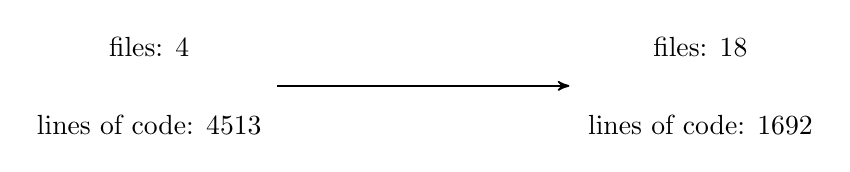
\begin{tikzpicture}[->,>=stealth',shorten >=1pt,auto,node distance=1cm,semithick]
    %% implementation
    \node[visible on=<1->] (original) {files: 4};
    \node[visible on=<1->] (originallocs) [below of=original] {lines of code: 4513};    

    \node[visible on=<2->] (after) [right of=original, xshift=6cm] {files: 18};
    \node[visible on=<2->] (afterlocs) [below of=after] {lines of code: 1692};

    \node[visible on=<2->] (a)  [below of=original, yshift=0.5cm, xshift=1.5cm] {};
    \node[visible on=<2->] (b)  [below of=after, yshift=0.5cm, xshift=-1.5cm] {};    
        
    \path[visible on=<2->] (a) edge (b);

  \end{tikzpicture}
\end{adjustbox}
\end{center}
\end{frame}

\begin{frame}[label={sec:org205fca0}]{Property Based Testing}
\begin{columns}
\begin{column}{0.48\columnwidth}
\onslide<+->
\onslide<+->
Proprety-Based Testing (PBT) is a great testing methodology.

\vspace{10pt}

Successful tools:
\begin{itemize}
\item Quviq QuickCheck
\item PropEr
\end{itemize}
\onslide<+->
\vspace{10pt}

These tools are great for testing pure functions.

\vspace{10pt}
\onslide<+->
They have mechanisms to test stateful programs.

\vspace{10pt}

PBT state-machines or models.

\vspace{10pt}

A PBT model works like an oracle.
\end{column}

\begin{column}{0.48\columnwidth}
\begin{figure}
\begin{adjustbox}{max width=\textwidth}
  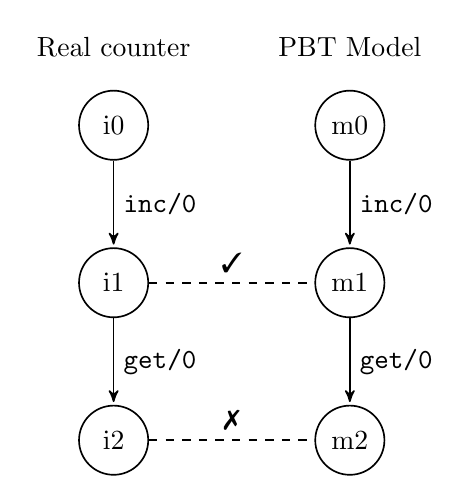
\begin{tikzpicture}[->,>=stealth',shorten >=1pt,auto,node distance=2cm,semithick]
    %% implementation
    \node[visible on=<5->] (il) {Real counter};
    \node[visible on=<5->] (ml) [right of=il, xshift=1cm] {PBT Model};

    \node[state, visible on=<6->] (i0) [below of=il, yshift=1cm] {i0};
    \node[state, visible on=<6->] (m0) [below of=ml, yshift=1cm] {m0};

    \node[state, visible on=<7->] (i1) [below of=i0] {i1};
    \node[state, visible on=<7->] (m1) [below of=m0] {m1};

    \node[state, visible on=<9->] (i2) [below of=i1] {i2};
    \node[state, visible on=<9->] (m2) [below of=m1] {m2};

    \path[visible on=<7->] (i0) edge node {\texttt{inc/0}} (i1);
    \path[visible on=<7->] (m0) edge node {\texttt{inc/0}} (m1);

    \path[visible on=<9->] (i1) edge node {\texttt{get/0}} (i2);
    \path[visible on=<9->] (m1) edge node {\texttt{get/0}} (m2);

    \path[-, dashed, visible on=<8->] (i1) edge node {$\cmark$} (m1);
    \path[-, dashed, visible on=<10->] (i2) edge node {$\xmark$} (m2);

  \end{tikzpicture}
\end{adjustbox}
\end{figure}
\end{column}
\end{columns}
\end{frame}

\begin{frame}[label={sec:orgdcfad98}]{Problems with PBT models}
\onslide<+->
\onslide<+->
Despite their proven effectiveness:
\begin{itemize}
\item Very slow adoption
\end{itemize}

\vspace{10pt}
\onslide<+->
Why?

\vspace{10pt}

\begin{enumerate}
\item Models are hard to reuse.
\item Bugs in models are hard to detect.
\item Generate cryptic errors.
\end{enumerate}
\onslide<+->
\vspace{10pt}

All these problems made models hard to write and maintain.
\end{frame}

\section{Introduction to Makina and running example}
\label{sec:org873ef6a}
\begin{frame}[label={sec:orgbf094da}]{Our solution: Makina}
\begin{columns}
\begin{column}{0.48\columnwidth}
Makina is a DSL for writing PBT models.
\onslide<+->
\onslide<+->

\vspace{10pt}

\vspace{1cm}
\begin{adjustbox}{max width=\textwidth}
  \begin{tikzpicture}[->,>=stealth',shorten >=1pt,auto,node distance=2cm,semithick]
    \node[inner sep=0pt] (makina) at (0,0) {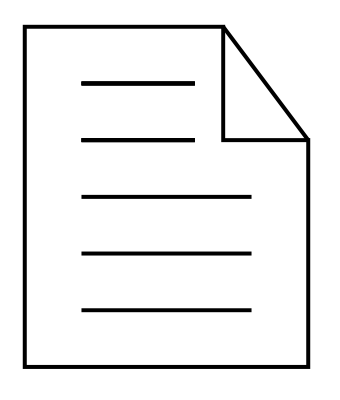
\includegraphics[width=.25\textwidth]{logos/file-cropped.png}};
    \node[inner sep=0pt] (proper) at (5,0) {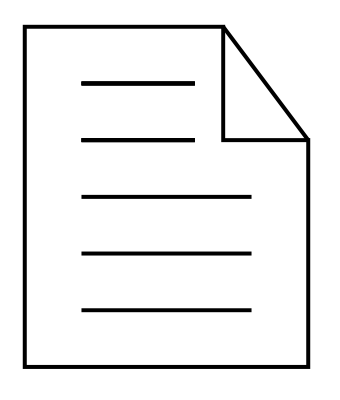
\includegraphics[width=.25\textwidth]{logos/file-cropped.png}};

    \path[->] (1,0) edge (4,0);

    \node (labelm) [below of=makina, yshift=0.5cm] {Makina model};
    \node (labelp) [below of=proper, yshift=0.5cm] {Proper/QuickCheck model};    
  \end{tikzpicture}
\end{adjustbox}
\end{column}

\begin{column}{0.48\columnwidth}
\onslide<3->
\begin{enumerate}
\item Models are hard to reuse.
\onslide<4->
\begin{itemize}
\item Modular reusable models. \vspace{10pt}
\end{itemize}
\onslide<3->
\item Bugs in models are hard to detect.
\onslide<5->
\begin{itemize}
\item Automatic type and specs generation. \vspace{10pt}
\end{itemize}
\onslide<3->
\item Errors are hard to understand.
\onslide<6->
\begin{itemize}
\item Automatic runtime-checks generation. \vspace{10pt}
\end{itemize}
\end{enumerate}
\end{column}
\end{columns}
\end{frame}

\begin{frame}[label={sec:orge4e06c2},fragile]{Makina: The Language}
 \begin{columns}
\begin{column}{0.48\columnwidth}
\onslide<+->
\lstset{language=elixir,label= ,caption= ,captionpos=b,numbers=none,style=display}
\begin{lstlisting}
defmodule Name do
  use Makina, [_option_]

  state [_attribute_]

  invariants [_invariants_]

  command _declaration_ do
    _command_body_
  end
end
\end{lstlisting}
\vspace{10pt}
\onslide<+->
\lstinline[language=elixir, style=display]~_option_~
\begin{itemize}
\item \lstinline[language=elixir, style=display]~extends: module()~
\item \lstinline[language=elixir, style=display]~extends: [module()]~
\item \lstinline[language=elixir, style=display]~implemented_by: module()~
\end{itemize}
\end{column}

\begin{column}{0.48\columnwidth}
\onslide<+->
\lstinline[language=elixir, style=display]~_attribute_~
\begin{itemize}
\item \lstinline[language=elixir, style=display]~name: expr~
\end{itemize}
\onslide<+->
\vspace{10pt}
\lstinline[language=elixir, style=display]~_declaration_~
\begin{itemize}
\item \lstinline[language=elixir, style=display]~name(arg1, ... , argN)~
\end{itemize}
\onslide<+->
\vspace{10pt}
\lstinline[language=elixir, style=display]~_command_body_~
\begin{itemize}
\item \lstinline[language=elixir, style=display]~pre~    \lstinline[language=elixir, style=display]~boolean()~
\item \lstinline[language=elixir, style=display]~args~   \lstinline[language=elixir, style=display]~generator()~
\item \lstinline[language=elixir, style=display]~call~   \lstinline[language=elixir, style=display]~return_type~
\item \lstinline[language=elixir, style=display]~next~   \lstinline[language=elixir, style=display]~[updates()]~
\item \lstinline[language=elixir, style=display]~post~   \lstinline[language=elixir, style=display]~boolean()~
\end{itemize}
\end{column}
\end{columns}
\end{frame}

\begin{frame}[label={sec:org9bd5038},fragile]{Ethereum Blockchain}
 Why Ethereum?
\begin{itemize}
\item It is a complex system.
\end{itemize}
\onslide<+->
\onslide<+->
\begin{center}
\begin{tabular}{lll}
API &  & \\
\hline
\lstinline[language=elixir, style=display]~accounts!/0~ & \lstinline[language=elixir, style=display]~accounts/0~ & \lstinline[language=elixir, style=display]~block_number!/0~\\
\lstinline[language=elixir, style=display]~call_transaction!/4~ & \lstinline[language=elixir, style=display]~call_transaction!/5~ & \lstinline[language=elixir, style=display]~call_transaction/4~\\
\lstinline[language=elixir, style=display]~client_version!/0~ & \lstinline[language=elixir, style=display]~client_version/0~ & \lstinline[language=elixir, style=display]~compile_solidity!/1~\\
\lstinline[language=elixir, style=display]~deploy!/3~ & \lstinline[language=elixir, style=display]~deploy!/4~ & \lstinline[language=elixir, style=display]~deploy/3~\\
\lstinline[language=elixir, style=display]~estimate_gas!/4~ & \lstinline[language=elixir, style=display]~estimate_gas!/5~ & \lstinline[language=elixir, style=display]~estimate_gas/4~\\
\lstinline[language=elixir, style=display]~estimate_gas_cost!/4~ & \lstinline[language=elixir, style=display]~estimate_gas_cost!/5~ & \lstinline[language=elixir, style=display]~estimate_gas_cost/4~\\
\lstinline[language=elixir, style=display]~gas_cost!/1~ & \lstinline[language=elixir, style=display]~gas_cost/1~ & \lstinline[language=elixir, style=display]~gas_price!/0~\\
\ldots{} & \ldots{} & \ldots{}\\
\end{tabular}
\end{center}


\begin{columns}
\begin{column}{0.48\columnwidth}
\onslide<+->
The properties to test:
\begin{enumerate}
\item Mining blocks.
\item Account access.
\item Transactions between accounts.
\end{enumerate}
\end{column}


\begin{column}{0.48\columnwidth}
\onslide<+->

How \lstinline[language=elixir, style=display]~Makina~ handles this complexity?
\end{column}
\end{columns}
\end{frame}

\section{Blocks model}
\label{sec:org088646a}
\begin{frame}[label={sec:org63d5421},fragile]{Mining blocks}
 \begin{columns}
\begin{column}{0.52\columnwidth}
\onslide<+->
\onslide<+->
The API:
\onslide<+->
\begin{center}
\begin{tabular}{ll}
Command & Returns\\
\hline
\lstinline[language=elixir, style=display]~mine/0~ & \lstinline[language=elixir, style=display]~:ok~\\
\lstinline[language=elixir, style=display]~block_number/0~ & \lstinline[language=elixir, style=display]~integer()~\\
\end{tabular}
\end{center}
\onslide<+->
\vspace{10pt}
\begin{enumerate}
\item create module.
\onslide<+->
\item import \lstinline[language=elixir, style=display]~Makina~.
\onslide<+->
\item define state.
\onslide<+->
\item define invariants.
\onslide<+->
\item define commands.
\end{enumerate}
\end{column}

\begin{column}{0.44\columnwidth}
\onslide<4->
\lstset{language=elixir,label= ,caption= ,captionpos=b,numbers=none,style=display}
\begin{lstlisting}
defmodule Blocks do #@ \onslide<5->
  use Makina
  #@ \onslide<6->
  state height: 0
  #@ \onslide<7->
  invariants non_neg_height: height > 0
  #@ \onslide<8->
  command block_number() do #@ \onslide<9->
    pre true #@ \onslide<10->
    args [] #@ \onslide<11->
    call Etherex.block_number #@ \onslide<12->
    next [] #@ \onslide<13->
    post height == result #@ \onslide<14->
  end
\end{lstlisting}
\end{column}
\end{columns}
\end{frame}

\begin{frame}[label={sec:org33634c1},fragile]{Mining blocks}
 \begin{columns}
\begin{column}{0.52\columnwidth}
The API:

\begin{center}
\begin{tabular}{ll}
Command & Returns\\
\hline
\lstinline[language=elixir, style=display]~mine/0~ & \lstinline[language=elixir, style=display]~:ok~\\
\lstinline[language=elixir, style=display]~block_number/0~ & \lstinline[language=elixir, style=display]~integer()~\\
\end{tabular}
\end{center}

\vspace{10pt}
\begin{enumerate}
\item create module.
\item import \lstinline[language=elixir, style=display]~Makina~.
\item define state.
\item define invariants.
\item define commands.
\end{enumerate}
\end{column}

\begin{column}{0.44\columnwidth}
\lstset{language=elixir,label= ,caption= ,captionpos=b,numbers=none,style=display}
\begin{lstlisting}
defmodule Blocks do
  use Makina, implemented_by: Etherex

  state height: 0

  invariants non_neg_height: height > 0

  command block_number() do
    post height == result
  end
  #@ \onslide<2->
  command mine() do
    next height: height + 1
  end
end
\end{lstlisting}
\end{column}
\end{columns}
\end{frame}

\begin{frame}[label={sec:org28fab94},fragile]{Running the test}
 \begin{columns}
\begin{column}{0.52\columnwidth}
\onslide<+->
\lstset{language=bash,label= ,caption= ,captionpos=b,numbers=none,style=shell}
\begin{lstlisting}
$ mix test
#@ \onslide<+->
Failed! After 1 tests.

Postcondition crashed:
** invariant "non_neg_height" check failed

block_number/0

Last state: %{height: 0}
\end{lstlisting}

\onslide<+->
This is a runtime check added by \lstinline[language=elixir, style=display]~Makina~!
\end{column}

\begin{column}{0.44\columnwidth}
\onslide<1->
\lstset{language=elixir,label= ,caption= ,captionpos=b,numbers=none,style=display}
\begin{lstlisting}
defmodule Blocks do
  use Makina, implemented_by: Etherex

  state height: 0

  invariants non_neg_height: height > 0

  command block_number() do
    post height == result
  end

  command mine() do
    next height: height + 1
  end
end
\end{lstlisting}
\end{column}
\end{columns}
\end{frame}

\begin{frame}[label={sec:orgd066579},fragile]{Fixing the model}
 \begin{columns}
\begin{column}{0.52\columnwidth}
\onslide<+->
\lstset{language=bash,label= ,caption= ,captionpos=b,numbers=none,style=shell}
\begin{lstlisting}
$ mix test

Failed! After 1 tests.

Postcondition crashed:
** invariant "non_neg_height" check failed

block_number/0

Last state: %{height: 0}
\end{lstlisting}

This is a runtime check added by \lstinline[language=elixir, style=display]~Makina~!
\end{column}

\begin{column}{0.44\columnwidth}
\lstset{language=elixir,label= ,caption= ,captionpos=b,numbers=none,style=display}
\begin{lstlisting}
defmodule Blocks do
  use Makina, implemented_by: Etherex

  state height: 0

  invariants non_neg_height: height >#@\only<2->{=} 0

  command block_number() do
    post height == result
  end

  command mine() do
    next height: height + 1
  end
end
\end{lstlisting}
\end{column}
\end{columns}
\end{frame}

\begin{frame}[label={sec:orgf96ccd1},fragile]{Running the test}
 \begin{columns}
\begin{column}{0.52\columnwidth}
\lstset{language=bash,label= ,caption= ,captionpos=b,numbers=none,style=shell}
\begin{lstlisting}
$ mix test #@\onslide<+->
#@\onslide<+->
..................................................
..................................................

OK, passed 100 tests

51.5 mine/0
48.5 block_number/0
\end{lstlisting}
\end{column}

\begin{column}{0.44\columnwidth}
\onslide<1->
\lstset{language=elixir,label= ,caption= ,captionpos=b,numbers=none,style=display}
\begin{lstlisting}
defmodule Blocks do
  use Makina, implemented_by: Etherex

  state height: 0

  invariants non_neg_height: height >= 0

  command block_number() do
    post height == result
  end

  command mine() do
    next height: height + 1
  end
end
\end{lstlisting}
\end{column}
\end{columns}
\end{frame}

\begin{frame}[label={sec:orgf214857},fragile]{Adding type information}
 \begin{columns}
\begin{column}{0.52\columnwidth}
\onslide<3->
\lstset{language=bash,label= ,caption= ,captionpos=b,numbers=none,style=shell}
\begin{lstlisting}
$ mix gradient

$
\end{lstlisting}

\vspace{10pt}
\onslide<4->
Something changes in \texttt{Etherex}\ldots{}

\vspace{10pt}

\onslide<5->
\lstset{language=bash,label= ,caption= ,captionpos=b,numbers=none,style=shell}
\begin{lstlisting}
$ mix gradient

The function call Etherex.block_number()
on line 8 is expected to have type integer()
but it has type
{:ok, quantity()} | {:error, error()}

$
\end{lstlisting}
\end{column}

\begin{column}{0.44\columnwidth}
\onslide<1->
\lstset{language=elixir,label= ,caption= ,captionpos=b,numbers=none,style=display, numbers=left}
\begin{lstlisting}
defmodule Blocks do
  use Makina, implemented_by: Etherex

  state height: 0 #@\only<2->{:: integer()}

  invariants non_neg_height: height >= 0

  command block_number()#@\only<2->{ :: integer()} do
    post height == result
  end

  command mine()#@\only<2->{ :: :ok} do
    next height: height + 1
  end
end
\end{lstlisting}
\end{column}
\end{columns}
\end{frame}

\begin{frame}[label={sec:orgbdac58e},fragile]{Adding documentation}
 \begin{columns}
\begin{column}{0.52\columnwidth}
\onslide<3->
\lstset{language=bash,label= ,caption= ,captionpos=b,numbers=none,style=shell}
\begin{lstlisting}
iex> h Blocks
#@\onslide<4->
Contains a Makina model called Blocks.

Checks blocks are mined correctly.

## Commands

- mine
- block_number

## State attributes

- height

## Invariants

- non_neg_height
\end{lstlisting}
\end{column}

\begin{column}{0.44\columnwidth}
\onslide<1->
\lstset{language=elixir,label= ,caption= ,captionpos=b,numbers=none,style=display}
\begin{lstlisting}
defmodule Blocks do
  use Makina, implemented_by: Etherex
  #@ \onslide<2->
  @moduledoc """
  Checks blocks are mined correctly.
  """ #@ \onslide<1->
  state height: 0 :: integer()

  invariants non_neg_height: height >= 0

  command block_number() :: integer() do #@ \onslide<2->
    @moduledoc "Gets the block number." #@ \onslide<1->
    post {:ok, height} == result
  end

  command mine() :: :ok do #@ \onslide<2->
    @moduledoc "Mines a new block." #@ \onslide<1->
    next height: height + 1
  end
end
\end{lstlisting}
\end{column}
\end{columns}
\end{frame}

\begin{frame}[label={sec:orgca0f064},fragile]{Adding documentation}
 \begin{columns}
\begin{column}{0.52\columnwidth}
\onslide<1->
\lstset{language=bash,label= ,caption= ,captionpos=b,numbers=none,style=shell}
\begin{lstlisting}
iex> h Blocks.Command.Mine
#@\onslide<2->
This module contains the functions necessary to
generate and execute the command mine.

Mines a new block.

## Definitions

- next
- call
- weight
- post
- args
- pre
\end{lstlisting}
\end{column}
\begin{column}{0.44\columnwidth}
\onslide<1->
\lstset{language=elixir,label= ,caption= ,captionpos=b,numbers=none,style=display}
\begin{lstlisting}
defmodule Blocks do
  use Makina, implemented_by: Etherex

  @moduledoc """
  Checks blocks are mined correctly.
  """
  state height: 0 :: integer()

  invariants non_neg_height: height >= 0

  command block_number() :: integer() do
    @moduledoc "Gets the block number."
    post height == result
  end

  command mine() :: :ok do
    @moduledoc "Mines a new block."
    next height: height + 1
  end
end
\end{lstlisting}
\end{column}
\end{columns}
\end{frame}

\begin{frame}[label={sec:org9860251},fragile]{Adding documentation}
 \begin{columns}
\begin{column}{0.52\columnwidth}
\onslide<1->
\lstset{language=bash,label= ,caption= ,captionpos=b,numbers=none,style=shell}
\begin{lstlisting}
iex> h Blocks.Command.Mine.post
#@\onslide<2->
This definition contains a predicate that should
be true after the execution of mine

## Available variables

### State

- state
- height

### Arguments

- arguments

### Result

- result
\end{lstlisting}
\end{column}

\begin{column}{0.44\columnwidth}
\onslide<1->
\lstset{language=elixir,label= ,caption= ,captionpos=b,numbers=none,style=display}
\begin{lstlisting}
defmodule Blocks do
  use Makina, implemented_by: Etherex

  @moduledoc """
  Checks blocks are mined correctly.
  """
  state height: 0 :: integer()

  invariants non_neg_height: height >= 0

  command block_number() :: integer() do
    @moduledoc "Gets the block number."
    post height == result
  end

  command mine() :: :ok do
    @moduledoc "Mines a new block."
    next height: height + 1
  end
end
\end{lstlisting}
\end{column}
\end{columns}
\end{frame}

\section{Accounts model}
\label{sec:org74e0b48}
\begin{frame}[label={sec:org9c2311c},fragile]{Account access}
 \begin{columns}
\begin{column}{0.28\columnwidth}
\onslide<+->
The API:

\begin{center}
\begin{tabular}{ll}
Command & Returns\\
\hline
\lstinline[language=elixir, style=display]~balance/1~ & \lstinline[language=elixir, style=display]~integer()~\\
\end{tabular}
\end{center}
\onslide<+->
\vspace{0.5cm}
\begin{enumerate}
\item create module.
\onslide<+->
\item import \lstinline[language=elixir, style=display]~Makina~.
\onslide<+->
\item define state.
\onslide<+->
\item define commands.
\end{enumerate}
\end{column}

\begin{column}{0.59\columnwidth}
\onslide<2->
\lstset{language=elixir,label= ,caption= ,captionpos=b,numbers=none,style=display}
\begin{lstlisting}
defmodule Accounts do #@\onslide<3->
  use Makina, implemented_by: Etherex
  #@\onslide<4->
  @type balances() :: %{address() => integer()}

  state accounts: Etherex.accounts() :: [address()],
	balances: Etherex.balances() :: balances()
  #@\onslide<5->
  command balance(account :: address()) :: integer() do
    pre accounts != []
    post balances[account] == result
  end #@\onslide<2->
end
\end{lstlisting}
\end{column}
\end{columns}
\end{frame}

\begin{frame}[label={sec:org461ac71},fragile]{Running the test}
 \begin{columns}
\begin{column}{0.28\columnwidth}
\onslide<+->
\lstset{language=bash,label= ,caption= ,captionpos=b,numbers=none,style=shell}
\begin{lstlisting}
$ mix test
#@\onslide<+->
** (Makina.Error) argument
`account` missing in command
get_balance
\end{lstlisting}
\vspace{20pt}
\onslide<+->
This is a runtime-check added by \lstinline[language=elixir, style=display]~Makina~!
\end{column}

\begin{column}{0.58\columnwidth}
\onslide<1->
\lstset{language=elixir,label= ,caption= ,captionpos=b,numbers=none,style=display}
\begin{lstlisting}
defmodule Accounts do
  use Makina, implemented_by: Etherex

  @type balances() :: %{address() => integer()}

  state accounts: Etherex.accounts() :: [address()],
	balances: Etherex.balances() :: balances()

  command balance(account :: address()) :: integer() do
    pre accounts != []
    post balances[account] == result
  end
end
\end{lstlisting}
\end{column}
\end{columns}
\end{frame}

\begin{frame}[label={sec:org0bfa6f6},fragile]{Fixing the model}
 \begin{columns}
\begin{column}{0.28\columnwidth}
\onslide<+->
\lstset{language=bash,label= ,caption= ,captionpos=b,numbers=none,style=shell}
\begin{lstlisting}
$ mix test

** (Makina.Error) argument
`account` missing in command
get_balance
\end{lstlisting}
\vspace{20pt}
This is a runtime-check added by \lstinline[language=elixir, style=display]~Makina~!
\end{column}

\begin{column}{0.58\columnwidth}
\onslide<1->
\lstset{language=elixir,label= ,caption= ,captionpos=b,numbers=none,style=display}
\begin{lstlisting}
defmodule Accounts do
  use Makina, implemented_by: Etherex

  @type balances() :: %{address() => integer()}

  state accounts: Etherex.accounts() :: [address()],
	balances: Etherex.balances() :: balances()

  command balance(account :: address()) :: integer() do
    args account: oneof(accounts)
    pre accounts != []
    post balances[account] == result
  end
end
\end{lstlisting}
\end{column}
\end{columns}
\end{frame}

\begin{frame}[label={sec:org58f7dca},fragile]{Running the test}
 \begin{columns}
\begin{column}{0.28\columnwidth}
\lstset{language=bash,label= ,caption= ,captionpos=b,numbers=none,style=shell}
\begin{lstlisting}
$ mix test #@\onslide<+->
#@\onslide<+->
.........................
.........................
.........................
.........................
OK, passed 100 tests

'100.0 get_balance/1
\end{lstlisting}
\end{column}

\begin{column}{0.58\columnwidth}
\onslide<1->
\lstset{language=elixir,label= ,caption= ,captionpos=b,numbers=none,style=display}
\begin{lstlisting}
defmodule Accounts do
  use Makina, implemented_by: Etherex
  @type balances() :: %{address() => integer()}

  state accounts: Etherex.accounts() :: [address()],
	balances: Etherex.balances() :: balances()

  command balance(account :: address()) :: integer() do
    args account: oneof(accounts)
    pre accounts != []
    post balances[account] == result
  end
end
\end{lstlisting}
\end{column}
\end{columns}
\end{frame}

\section{Transactions model}
\label{sec:orge274ddf}
\begin{frame}[label={sec:org1bc1e39},fragile]{Generating transactions}
 \begin{columns}
\begin{column}{0.48\columnwidth}
\onslide<+->
\onslide<+->
The API to generate and check transactions:
\onslide<+->
\begin{center}
\begin{tabular}{lll}
Command & Returns & Implemented\\
\hline
\lstinline[language=elixir, style=display]~mine/0~ & \lstinline[language=elixir, style=display]~:ok~ & \(\checkmark\)\\
\lstinline[language=elixir, style=display]~block_number/0~ & \lstinline[language=elixir, style=display]~integer()~ & \(\checkmark\)\\
\lstinline[language=elixir, style=display]~get_balance/1~ & \lstinline[language=elixir, style=display]~integer()~ & \(\checkmark\)\\
\lstinline[language=elixir, style=display]~transfer/3~ & \lstinline[language=elixir, style=display]~hash()~ & \\
\end{tabular}
\end{center}
\onslide<+->
We can compose \lstinline[language=elixir, style=display]~Blocks~ and \lstinline[language=elixir, style=display]~Accounts~!
\onslide<+->
\lstset{language=elixir,label= ,caption= ,captionpos=b,numbers=none,style=display}
\begin{lstlisting}
defmodule Transactions do
  use Makina,
    extends: [Blocks, Accounts],
    implemented_by: Etherex
end
\end{lstlisting}
\onslide<+->
Generates a model \lstinline[language=elixir, style=display]~Transactions.Composed~.
\end{column}

\begin{column}{0.48\columnwidth}
\onslide<+->
\lstset{language=bash,label= ,caption= ,captionpos=b,numbers=none,style=shell}
\begin{lstlisting}
iex(1)> h Transactions.Composed
#@\onslide<+->
# Transactions.Composed

## Commands

- mine stored
- get_balance
- block_number

## State attributes

- height
- balances
- accounts

## Invariants

- non_neg_height

\end{lstlisting}
\end{column}
\end{columns}
\end{frame}

\begin{frame}[label={sec:orgc4c71e4},fragile]{Generating transactions}
 \begin{columns}
\begin{column}{0.44\columnwidth}
\onslide<+->
\lstinline[language=elixir, style=display]~Transactions extends: Transactions.Composed~.
\vspace{10pt}

\onslide<+->
\begin{center}
\begin{tabular}{ll}
Command & Returns\\
\hline
\texttt{transfer/3} & \texttt{hash()}\\
\end{tabular}
\end{center}
\end{column}
\begin{column}{0.52\columnwidth}
\onslide<1->
\lstset{language=elixir,label= ,caption= ,captionpos=b,numbers=none,style=display}
\begin{lstlisting}
defmodule Transactions do
  use Makina,
    implemented_by: Etherex,
    extends: [Accounts, Blocks]
  #@\onslide<2->
  command transfer(from, to, value) :: hash() do
    pre accounts != []
    args from: oneof(accounts),
	 to: oneof(accounts),
	 value: pos_integer()
    next balances: update(balances, from, to, value)
  end    #@\onslide<1->
end
\end{lstlisting}
\end{column}
\end{columns}
\end{frame}

\begin{frame}[label={sec:orgab365cd},fragile]{Running the test}
 \begin{columns}
\begin{column}{0.44\columnwidth}
\lstset{language=bash,label= ,caption= ,captionpos=b,numbers=none,style=shell}
\begin{lstlisting}
$ mix test #@\onslide<+->
#@\onslide<+->
transfer("0xffcf8fdee72ac11",
	 "0x90f8bf6a479f320",
	 1)
block_number()

Postcondition failed.

block_number() -> 1

Last state: %{height: 0, ...}
\end{lstlisting}
\end{column}

\begin{column}{0.52\columnwidth}
\onslide<1->
\lstset{language=elixir,label= ,caption= ,captionpos=b,numbers=none,style=display}
\begin{lstlisting}
defmodule Transactions do
  use Makina,
    implemented_by: Etherex,
    extends: [Accounts, Blocks]

  command transfer(from, to, value) :: hash() do
    pre accounts != []
    args from: oneof(accounts),
	 to: oneof(accounts),
	 value: pos_integer()
    next balances: update(balances, from, to, value)
  end
end
\end{lstlisting}
\end{column}
\end{columns}
\end{frame}

\begin{frame}[label={sec:org8af31fb},fragile]{Fixing the model}
 \begin{columns}
\begin{column}{0.44\columnwidth}
\lstset{language=bash,label= ,caption= ,captionpos=b,numbers=none,style=shell}
\begin{lstlisting}
$ mix test

transfer("0xffcf8fdee72ac11",
	 "0x90f8bf6a479f320",
	 1)
block_number()

Postcondition failed.

block_number() -> 1

Last state: %{height: 0, ...}
\end{lstlisting}
\end{column}

\begin{column}{0.52\columnwidth}
\onslide<1->
\lstset{language=elixir,label= ,caption= ,captionpos=b,numbers=none,style=display}
\begin{lstlisting}
defmodule Transactions do
  use Makina,
    implemented_by: Etherex,
    extends: [Accounts, Blocks]

  command transfer(from, to, value) :: hash() do
    pre accounts != []
    args from: oneof(accounts),
	 to: oneof(accounts),
	 value: pos_integer()
    next height: height + 1,
	 balances: update(balances, from, to, value)
  end
end
\end{lstlisting}
\end{column}
\end{columns}
\end{frame}

\begin{frame}[label={sec:org727d3b8},fragile]{Running the test}
 \begin{columns}
\begin{column}{0.44\columnwidth}
\onslide<+->
\lstset{language=bash,label= ,caption= ,captionpos=b,numbers=none,style=shell}
\begin{lstlisting}
$ mix test #@\onslide<+->

transfer("0x90f8bf6a479f320",
	 "0xffcf8fdee72ac11",
	 1),
get_balance("0x90f8bf6a479f320")

Postcondition failed.

get_balance("0x90f8bf6a479f320") -> 979000

Last state: %{
    balances: %{
	"0x90f8bf6a479f320" => 1000000
	.. }
    .. }
\end{lstlisting}
\end{column}

\begin{column}{0.52\columnwidth}
\onslide<1->
\lstset{language=elixir,label= ,caption= ,captionpos=b,numbers=none,style=display}
\begin{lstlisting}
defmodule Transactions do
  use Makina,
    implemented_by: Etherex,
    extends: [Accounts, Blocks]

  command transfer(from, to, value) :: hash() do
    pre accounts != []
    args from: oneof(accounts),
	 to: oneof(accounts),
	 value: pos_integer()
    next height: height + 1,
	 balances: update(balances, from, to, value)
  end
end
\end{lstlisting}
\end{column}
\end{columns}
\end{frame}

\begin{frame}[label={sec:orgb702cbb},fragile]{Fixing the model}
 \begin{columns}
\begin{column}{0.44\columnwidth}
To fix this error we need to extract the gas cost after producing a transaction.
\onslide <+->
\onslide <+->
\vspace{10pt}


Model execution is performed in two phases:
\begin{enumerate}
\item Generation of the command sequence.
\item Real execution of the test.
\end{enumerate}
\onslide <+->
\vspace{10pt}

PBT libraries solve this documenting:
\begin{itemize}
\item symbolic state: state of the model during phase 1.
\item dynamic state: state of the model during phase 2.
\end{itemize}
\end{column}

\begin{column}{0.52\columnwidth}
\onslide<1->
\lstset{language=elixir,label= ,caption= ,captionpos=b,numbers=none,style=display}
\begin{lstlisting}
defmodule Transactions do
  use Makina,
    implemented_by: Etherex,
    extends: [Accounts, Blocks]

  command transfer(from, to, value) :: hash() do
    pre accounts != []
    args from: oneof(accounts),
	 to: oneof(accounts),
	 value: pos_integer()
    next height: height + 1,
	 balances: update(balances, from, to, value)
  end
end
\end{lstlisting}
\end{column}
\end{columns}
\end{frame}

\begin{frame}[label={sec:orgd263921},fragile]{Fixing the model}
 \begin{columns}
\begin{column}{0.44\columnwidth}
\onslide <+->
\onslide <+->
\lstinline[language=elixir, style=display]~Makina~ makes the difference between symbolic and dynamic explicit.

\vspace{10pt}
\onslide <+->
Provides two mechanisms to add information about symbolic state:
\begin{itemize}
\item \lstinline[language=elixir, style=display]~symbolic(t)~ type.
\item \lstinline[language=elixir, style=display]~symbolic(expr)~ macro.
\end{itemize}

\onslide <+->
Rules on symbolic state:
\begin{itemize}
\item An attribute with a symbolic type cannot be inspected in \lstinline[language=elixir, style=display]~next~.
\item If we need to update a symbolic attribute we should use symbolic macro.
\end{itemize}

\vspace{10pt}
\onslide <+->
To fix our model we need
\begin{enumerate}
\item Add symbolic attributes to the state.
\onslide <7->
\item Store and update symbolic attributes.
\end{enumerate}
\end{column}

\begin{column}{0.52\columnwidth}
\onslide<1->
\vspace{-10pt}
\lstset{language=elixir,label= ,caption= ,captionpos=b,numbers=none,style=display}
\begin{lstlisting}
defmodule Transactions do
  use Makina,
    implemented_by: Etherex,
    extends: [Accounts, Blocks]
  #@ \onslide<6->
  state transactions: [] :: [symbolic(hash())]
	balances: super() :: symbolic(balances)
  #@ \onslide<1->
  command transfer(from, to, value) :: hash() do
    pre accounts != []
    args from: oneof(accounts),
	 to: oneof(accounts),
	 value: pos_integer()
    next height: height + 1,
	 #@\onslide<8->{transactions: [result | transactions],}
	 balances: update(balances, from, to, value)
		       #@\onslide<8->{|> symbolic()}
  end

  command get_balance() do
    pre transactions == []
  end
end
\end{lstlisting}
\end{column}
\end{columns}
\end{frame}

\begin{frame}[label={sec:org5f23036},fragile]{Fixing the model}
 \begin{columns}
\begin{column}{0.38\columnwidth}
We import \lstinline[language=elixir, style=display]~Transactions~ model using \lstinline[language=elixir, style=display]~:extends~.

\vspace{10pt}
\onslide <+->
\onslide <+->
We add a command that gets the cost of a transaction.
\end{column}

\begin{column}{0.58\columnwidth}
\onslide <1->
\lstset{language=elixir,label= ,caption= ,captionpos=b,numbers=none,style=display}
\begin{lstlisting}
defmodule Transactions.GasCost do
  use Makina, extends: Transactions
  #@ \onslide<3->
  command gas_cost(hash :: hash())
      :: {address(), quantity()} do
    pre transactions != []
    args hash: oneof(transactions)
    next transactions: List.delete(transactions, hash),
	 balances: update_gas(balances, result)
		   |> symbolic()
    end     #@ \onslide<1->
  end
end
\end{lstlisting}
\end{column}
\end{columns}
\end{frame}

\begin{frame}[label={sec:org94c69e0},fragile]{Running the test}
 \begin{columns}
\begin{column}{0.38\columnwidth}
\onslide <+->
\lstset{language=bash,label= ,caption= ,captionpos=b,numbers=none,style=shell}
\begin{lstlisting}
$ mix test
#@ \onslide<+->
.........................
.........................
.........................
.........................

OK, passed 100 tests

'25.5 mine/0
'24.9 block_number/0
'23.6 transfer/3
'14.3 gas_cost/1
'11.8 get_balance/1
\end{lstlisting}
\end{column}

\begin{column}{0.58\columnwidth}
\onslide <1->
\lstset{language=elixir,label= ,caption= ,captionpos=b,numbers=none,style=display}
\begin{lstlisting}
defmodule Transactions.GasCost do
  use Makina, extends: Transactions

  command gas_cost(hash :: hash())
      :: {address(), quantity()} do
    pre transactions != []
    args hash: oneof(transactions)
    next transactions: List.delete(transactions, hash),
	 balances: update_gas(balances, result)
		   |> symbolic()
    end
  end
end
\end{lstlisting}
\end{column}
\end{columns}
\end{frame}
\section{Conclusions}
\label{sec:org0b609be}
\begin{frame}[label={sec:org7d49b79},fragile]{Results}
 \onslide<+->
\onslide<+->

\begin{center}
\begin{tabular}{ll}
Problem on PBT models & \lstinline[language=elixir, style=display]~Makina~ solution\\
\hline
 & \\
Hard to reuse. & Modular and composable models.\\
 & \\
Bugs are hard to detect. & Type and specs generation.\\
 & \\
Generate cryptic errors. & Automatic runtime-checks.\\
\end{tabular}
\end{center}

\vspace{10pt}

\onslide<+->

\begin{center}
\begin{tabular}{ll}
Before \lstinline[language=elixir, style=display]~Makina~ & After \lstinline[language=elixir, style=display]~Makina~\\
\hline
 & \\
4 files 4513 lines & 18 files 1692 lines\\
\end{tabular}
\end{center}
\end{frame}

\begin{frame}[label={sec:org47f3ce3}]{Links}
\begin{columns}
\begin{column}{0.78\columnwidth}
Makina library:
\begin{itemize}
\item \url{https://gitlab.com/babel-upm/makina/makina/}
\end{itemize}
\vspace{10pt}
Makina examples:
\begin{itemize}
\item \url{https://gitlab.com/babel-upm/makina/examples/}
\end{itemize}
\vspace{10pt}
Etherex library:
\begin{itemize}
\item \url{https://gitlab.com/babel-upm/blockchain/etherex}
\end{itemize}
\vspace{10pt}
\end{column}
\end{columns}
\end{frame}
\end{document}